\documentclass[10pt]{beamer}
\usepackage[utf8]{inputenc}
\usepackage{xeCJK}
\usepackage{graphicx}
\usepackage {mathtools}
\usepackage{utopia} %font utopia imported
\usetheme{CambridgeUS}
\usecolortheme{dolphin}

% set colors
\definecolor{myNewColorA}{RGB}{126,12,110}
\definecolor{myNewColorB}{RGB}{165,85,154}
\definecolor{myNewColorC}{RGB}{203,158,197}
\setbeamercolor*{palette primary}{bg=myNewColorC}
\setbeamercolor*{palette secondary}{bg=myNewColorB, fg = white}
\setbeamercolor*{palette tertiary}{bg=myNewColorA, fg = white}
\setbeamercolor*{titlelike}{fg=myNewColorA}
\setbeamercolor*{title}{bg=myNewColorA, fg = white}
\setbeamercolor*{item}{fg=myNewColorA}
\setbeamercolor*{caption name}{fg=myNewColorA}
\usefonttheme{professionalfonts}
\usepackage{natbib}
\usepackage{hyperref}
\newtheorem{exmp}{Example}[section]
%------------------------------------------------------------
\titlegraphic{
\includegraphics[height=1.5cm]{logo.png}}

\setbeamerfont{title}{size=\large}
\setbeamerfont{subtitle}{size=\small}
\setbeamerfont{author}{size=\small}
\setbeamerfont{date}{size=\small}
\setbeamerfont{institute}{size=\small}
\title[Universitat de Valencia]{Sphere packings}
\subtitle{Introduction}
\author[Análisis matemático y aplicaciones]{Roylan Martinez}

\institute[ ]{Universitat de València}
\date[February 23, 2023]
{Valencia, Spain}

%------------------------------------------------------------
%This block of commands puts the table of contents at the 
%beginning of each section and highlights the current section:
%\AtBeginSection[]
%{
%  \begin{frame}
%    \frametitle{Contents}
%    \tableofcontents[currentsection]
%  \end{frame}
%}
\AtBeginSection[]{
  \begin{frame}
  \vfill
  \centering
  \begin{beamercolorbox}[sep=8pt,center,shadow=true,rounded=true]{title}
    \usebeamerfont{title}\insertsectionhead\par%
  \end{beamercolorbox}
  \vfill
  \end{frame}
}
%------------------------------------------------------------

\begin{document}

%The next statement creates the title page.
\frame{\titlepage}
\begin{frame}
\frametitle{Contents}
\tableofcontents
\end{frame}
%------------------------------------------------------------
\section{Sphere packing original problem}

\begin{frame}{Sphere packing original problem}
    \frametitle{Sphere packing original problem}
    
    
     What's the densest packing of spheres into Euclidean space?

    \begin{figure}[t]
    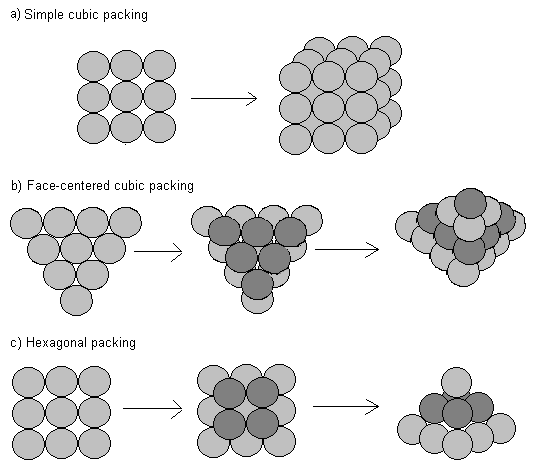
\includegraphics[width=5cm]{1.png}
    \centering
    \caption{Packaging examples \cite{arnold2000cannon}}
    \end{figure}
\end{frame}

\section{Density function}


\begin{frame}{Density function}
    \frametitle{Density function of spheres packaging in $n$-dimensional Euclidean space}
    
    Foremost, by definition it will be given that $x \in \mathbb{R}^d$, $r \in \mathbb{R}_{>0}$ and $B_d(x, r)$ will be the open ball in $\mathbb{R}$ with center $x$ and radius $r$. Besides, $X \subset \mathbb{R}^d$ will be all the discrete points such that $\forall x, y \in X: x \neq y: ||x-y|| \geq 2$. Then: 
    
    \begin{equation} \label{1}
    \begin{split}
        \mathcal{P} = \bigcup_{x \in X} B_d(x, 1) 
    \end{split}
    \end{equation}

will be defined to be a sphere packing, because we assume $X$ is not necessarily a $\mathbb{R}^d$-lattice. Subsequently, the density function $\Delta_\mathcal{P}(r)$ will be introduced. 

    \begin{definition}[Density function] 
    
    The density function $\Delta_\mathcal{P}(r)$ will be defined as: 
    
    
    \begin{equation} \label{2}
    \begin{split}
        \Delta_\mathcal{P} := \frac{Vol(\mathcal{P} \cap B_d(0, r))}{Vol(B_d(0, r))}, r > 0.
    \end{split}
    \end{equation}
\end{definition}
\end{frame}

\begin{frame}{Introduction}
    \frametitle{Density function of spheres packaging in $n$-dimensional Euclidean space}
    
    Besides, the density  of a packing $\mathcal{P}$ will be defined as the limit superior of $\Delta_\mathcal{P}(r)$, subsequently: 
    
    \begin{equation} \label{3}
    \begin{split}
        \Delta _\mathcal{P} := \limsup_{r \rightarrow \infty} \Delta _\mathcal{P}(r).
    \end{split}
    \end{equation}
    
    The number we are interested is therefore the supremum of all the given possible packing densities \cite{viazovska2017sphere}, i.e: 
    
    \begin{equation} \label{4}
    \begin{split}
        \Delta_d := \sup_{\mathcal{P} \subset \mathbb{R}^d} \Delta_\mathcal{P}
    \end{split}
    \end{equation}

\end{frame}

\section{Sphere packing in $\mathbb{R}$}

\begin{frame}{Sphere packing in $\mathbb{R}$}
    \frametitle{Sphere packing in $1$-dimensional Euclidean space}
    
    Given a $1$-sphere in a $1$-dimensional Euclidean space, it is easy to see that $\Delta_d = 1$
    \begin{figure}[t]
    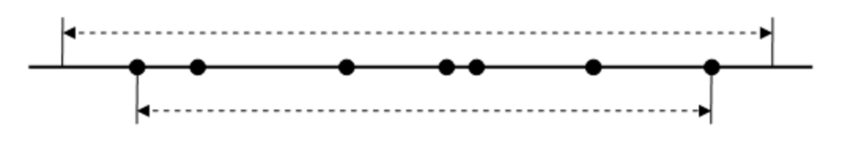
\includegraphics[width=8cm]{0.png}
    \centering
    \caption{The density of $1$-spheres }
    \end{figure}
\end{frame}

\section{Sphere packing in $\mathbb{R}^2$}

\begin{frame}{Sphere packing in $\mathbb{R}^2$}
    \frametitle{Sphere packing in $2$-dimensional Euclidean space}
    
    The case of a $2$-sphere is a little bit more complex than in the $1$-dimension case. Given a $2$-sphere in a $2$-dimensional Euclidean space, it was proved that $\Delta_d = \frac{1}{6} \pi \sqrt{3} \approx 0.91$. by \cite{thue1911dichteste}---and it is the one referenced in \cite{viazovska2017sphere}---, however, the proof is considerably more complex than the one given in by \cite{chang2010simple} and therefore this last one will be used instead. 
    
    
    \begin{block}{Lemma 1}
    Let $\theta$ be the largest internal angle of a given triangle $\Delta ABC$ in a Delaunay
triangulation for a saturated circle configuration $C$. Then

    \begin{equation} \label{4}
    \begin{split}
        \frac{\pi}{3} \leq \theta < \frac{2 \pi}{3}.
    \end{split}
    \end{equation}
    \end{block}
    
    \begin{block}{Proof Lemma 1}
    The largest internal angle is always equal or bigger than $\frac{\pi}{3}$. So, without loss of generality if assumed $\theta \geq \frac{2\pi}{3} > \frac{\pi}{3}$, then let $A$ the smallest internal angle. We will have that $\sin(A)$ and $\overline{BC} \geq 2$. 
    \vspace{1cm}
    \end{block}
\end{frame}

\begin{frame}{Sphere packing in $\mathbb{R}^2$}
    \frametitle{Sphere packing in $2$-dimensional Euclidean space}
    
    \begin{block}{}
    
 We will assume $R$ is the circumradius of $\overline{ABC}$. Then, using the sine law we will get: 
    
    \begin{equation} \label{5}
    \begin{split}
        2 R = \frac{\overline{BC}}{\sin A} \geq \frac{2}{\sin A} \geq 4. 
    \end{split}
    \end{equation}
    
    Consequently the circumradius of $\Delta ABC$ can be added to the circle configuration $\mathcal{C}$, therefore we get: 
    \begin{equation} \label{6}
    \begin{split}
        \theta < \frac{2 \pi}{3}. \text{ Q.E.D.}
    \end{split}
    \end{equation}
    Therefore, the density of a triangle $\Delta ABC$ in a Delaunnay triangulation for a satured circle configuration $\mathcal{C}$ is given by:
    
    \begin{equation} \label{6.1}
    \begin{split}
        \frac{\frac{1}{2} A + \frac{1}{2} + B \frac{1}{2} C}{\text{area of } \Delta ABC} = \frac{\frac{\pi}{2}}{\text{area of } \Delta ABC}.
    \end{split}
    \end{equation}
    
    \end{block}
\end{frame}

\begin{frame}{Sphere packing in $\mathbb{R}^2$}
    \frametitle{Sphere packing in $2$-dimensional Euclidean space}
    
    \begin{block}{Lemma 2}
    The density of a triangle $\Delta ABC$ in a Delaunay triangulation for a satred circle configuration $C$, holds that $C \leq \pi / \sqrt{12}$. The equality holds only for the regular triangle with side-length $2$.
    \end{block}
    
    \begin{block}{Proof Lemma 2}
    Let's assume, without loss of generality, that $B$ is the largest internal angle of $\Delta ABC$. Then, by the first lemma, 
    
    \begin{equation} \label{6.3}
    \begin{split}
        \\ \text{area of } \Delta ABC = \frac{1}{2} \overline{AB} \cdot \overline{BC} \cdot \sin B \geq \frac{1}{2} \cdot 2 \cdot 2 \cdot \frac{\sqrt{3}}{2} = \sqrt{3} &
        \\ \implies \text{density of } \Delta ABC = \frac{\pi / 2}{\text{area of } \Delta ABC} \leq \frac{\pi}{\sqrt{12}}. & 
    \end{split} 
    \end{equation}
    
    If $\Delta ABC$ is a regular triangle with side-length $ = 2$ then it becomes a equality
    
    \end{block}
\end{frame}

\section{Simulations of sphere packing in $\mathbb{R}^2$}
\begin{frame}{Simulations}


Simulations in Python for $\mathbb{R}^2$.

\begin{figure}[t]
    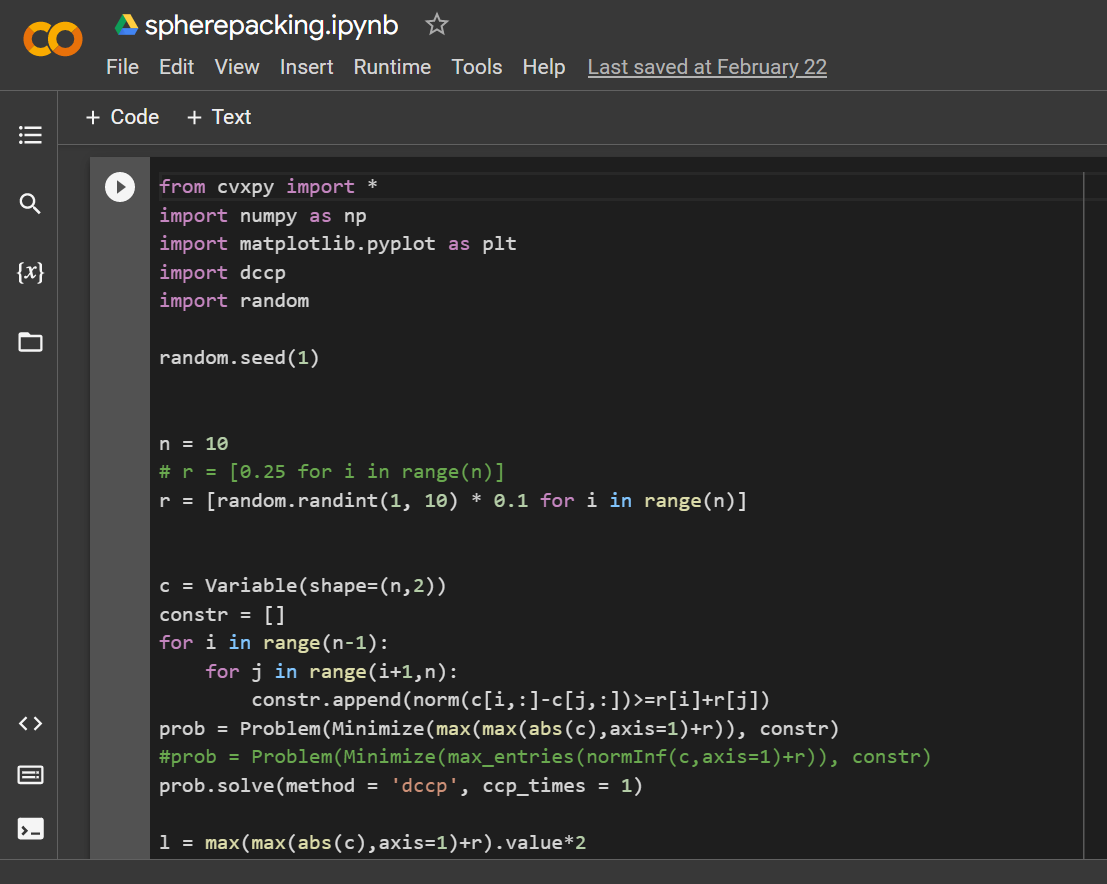
\includegraphics[width=5cm]{code.png}
    \centering
    \caption{Collab platform}
    \end{figure}
    
\href{https://colab.research.google.com/drive/1C3HyFZRLydt18go0Bki9KnKzpY5WKpE3?usp=sharing}{\LARGE\beamergotobutton{SIMULATIONS}}
\end{frame}

\section{Sphere packing in $\mathbb{R}^3$}
\begin{frame}{Sphere packing in $\mathbb{R}^3$}

    
    \begin{block}{Lemma 3}
    
    The highest density amongst all possible $3$-dimensional lattice packings of spheres in $\mathbb{R}^3$ corresponds to: 

  \begin{equation} \label{6.4}
    \begin{split}
        \Delta_3 := \frac{\pi}{\sqrt{18}} \approx 0.74.
    \end{split}
    \end{equation}
    
    \end{block}
    
    
    The proof of Lemma 2 was originally solved in 1998, however it was 250 pages long, with 3 gigabytes of calculations and after 4 years, journal referees said that they were "$99\%$ certain" his proof was right. The journal published his paper, but Hales turned to giving a fully rigorous computerized proof of the Kepler Conjecture.   He organized a team to do this named the "Flyspeck project" and they finished in 2014. The proof is $30$ pages long using a "Proof assistant" but it is still quite complex. \cite{hales2017formal}
    
\end{frame}



\section{Close-packing of equal spheres
 $\mathbb{R}^3$}
\begin{frame}{Close-packing of equal spheres
 $\mathbb{R}^3$}

    \begin{block}{Definition: Face-centred cubic}
    
    FCC is a face-centred cubic close packing structure of lattices. It is a space-efficient composition of crystal structures. The coordination number of this structure is 12, while the number of atoms per unit cell is 4. Here, the coordination number is the number of atoms the unit cell touches. Importantly, this structure efficiently occupies $74\%$. of the space; thus, the empty space is $26\%$.
    
    \begin{figure}[t]
    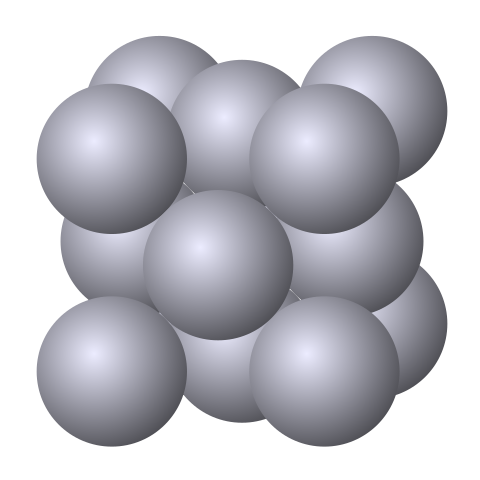
\includegraphics[width=3cm]{hh1.png}
    \centering
    \caption{Collab platform}
    \end{figure}
    
    \end{block}
 

\end{frame}

\begin{frame}{Close-packing of equal spheres $\mathbb{R}^3$}
    \begin{block}{Definition: Hexagonal close packing}
    
    HCP is a hexagonal close packing structure of lattices. It is also a space-efficient composition of crystal structures.  The coordination number of this structure is 2, while the number of atoms per unit cell is $6$. The structure occupies $74\%$ of total space; thus, the empty space is  $26\%$. Here, HCP layers cycle among two layers. That means; the third layer of the structure is similar to the first layer.


    
    \begin{figure}[t]
    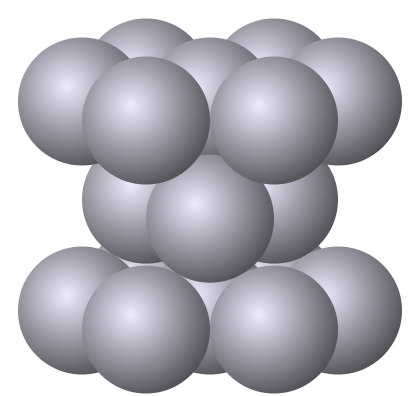
\includegraphics[width=3cm]{hh2.png}
    \centering
    \caption{Collab platform}
    \end{figure}
    \end{block}
\end{frame}

\begin{frame}{Contrast}
    \begin{block}{Hexagonal close packing contrast: HCC and FCC}

    
    \begin{figure}[t]
    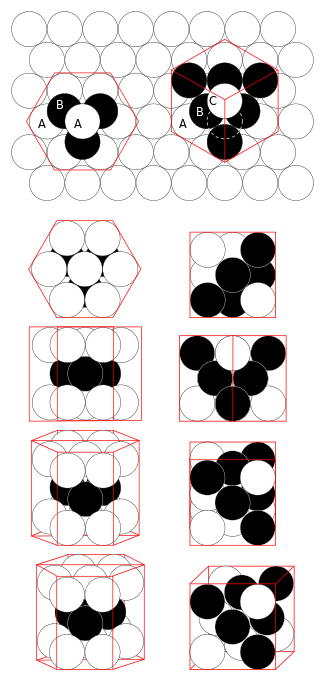
\includegraphics[width=3cm,  angle =90]{contrast.png}
    \centering
    \caption{Contrast in contained space}
    \end{figure}
    \end{block}
\end{frame}
    

\section{Sphere packing in $\mathbb{R}^8$}
\begin{frame}{Sphere packing in $\mathbb{R}^8$}

\begin{block}{Lemma 4}
    
    The highest density amongst all possible $8$-dimensional lattice packings of spheres in $\mathbb{R}^3$ corresponds to: 

  \begin{equation} \label{6.4}
    \begin{split}
        \Delta_8 := \frac{\pi^4}{384} \approx 0.25.
    \end{split}
    \end{equation}
    
    Consequently, the $E^8$ lattice packing is the densest sphere packing in $\mathbb{R}^8$ \cite{viazovska2017sphere}.
    
    \end{block}
    
    

\end{frame}

\begin{frame}{Sphere packing in $\mathbb{R}^8$}

\begin{block}{Linear programming bounds for sphere packing}
    
    The idea is first to define the following Fourier transformation of $f$:

  \begin{equation} \label{6.4}
    \begin{split}
        \tilde{f}(t) = \int_{\mathbb{R^n}} f(x)e^{2 \pi \langle x, t \rangle} dx.
    \end{split}
    \end{equation}
    
    Then, using the theorem of Cohn-Elkies, if we suppose $f: \mathbb{R}^n \rightarrow \mathbb{R}$ is a Schwartz function with the following properties:
    
    
    \begin{enumerate}
    \item $\text{1. } f(0) = \tilde{f}(0) = 1.$
    \item $\text{2. } f(x) \leq 0 \text{ for } |x| \geq r$
    \item $\text{3. } \tilde{f}(t) \forall t$
\end{enumerate}

If the conditions are done then the density of any sphere packing in $\mathbb{R}^8$ is bounded avobe by: 

\begin{equation} \label{6.4}
    \begin{split}
        vol(B_n)(\frac{r}{2})^n
    \end{split}
    \end{equation}
    
    \end{block}
    
    

\end{frame}


\begin{frame}{Sphere packing in $\mathbb{R}^8$}

Note then is a linear programming bound, by scaling $f$ appropriately we can check if the conditions are fulfilled, s the density is bounded by $2^{-n}vol(B_n)f(0)$. Note that the constraints and objective function given are linear in $f$ and therefore it is a linear convex program. 

    \begin{figure}[t]
    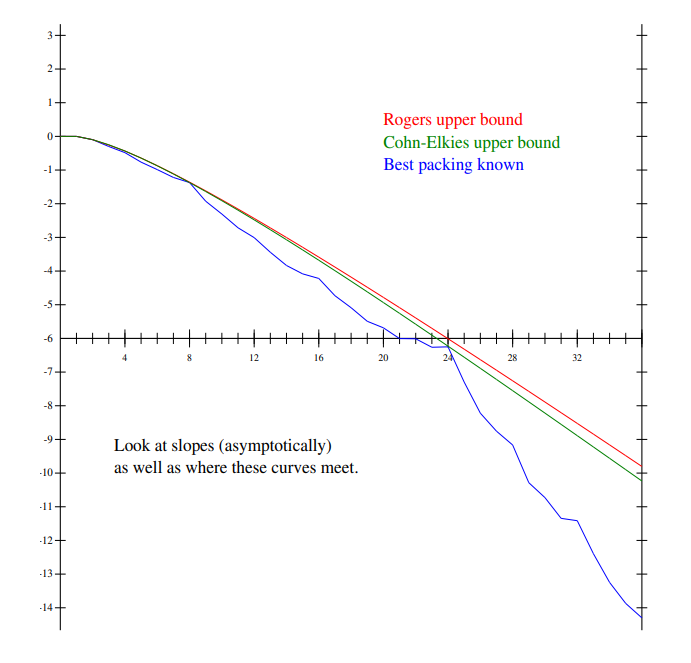
\includegraphics[width=3cm]{maplog.png}
    \centering
    \caption{$\log$(density) vs. dimension}
    \end{figure}


    
    

\end{frame}


\begin{frame}{Desired functions}

Let $\Lambda$ be $E_8$ and $r_0, r_1, \dots$ its nonzero vector lengths (square roots of the even natural numbers). To have a right upper bound that matches $\Lambda$, it is necessary to get a function $f$ that looks like this:

    \begin{figure}[t]
    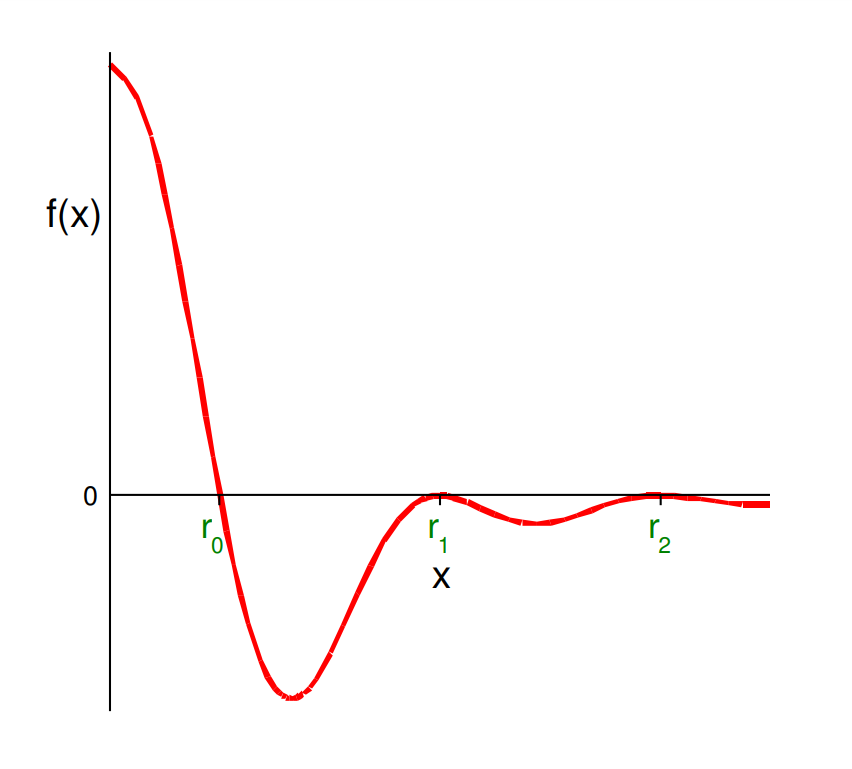
\includegraphics[width=3cm]{f1.png}
    \centering
    \caption{How $f$ should look like}
    \end{figure}


    
    

\end{frame}

\begin{frame}{Desired functions}

On the other hand, $\tilde{f}$ should look like this: 

    \begin{figure}[t]
    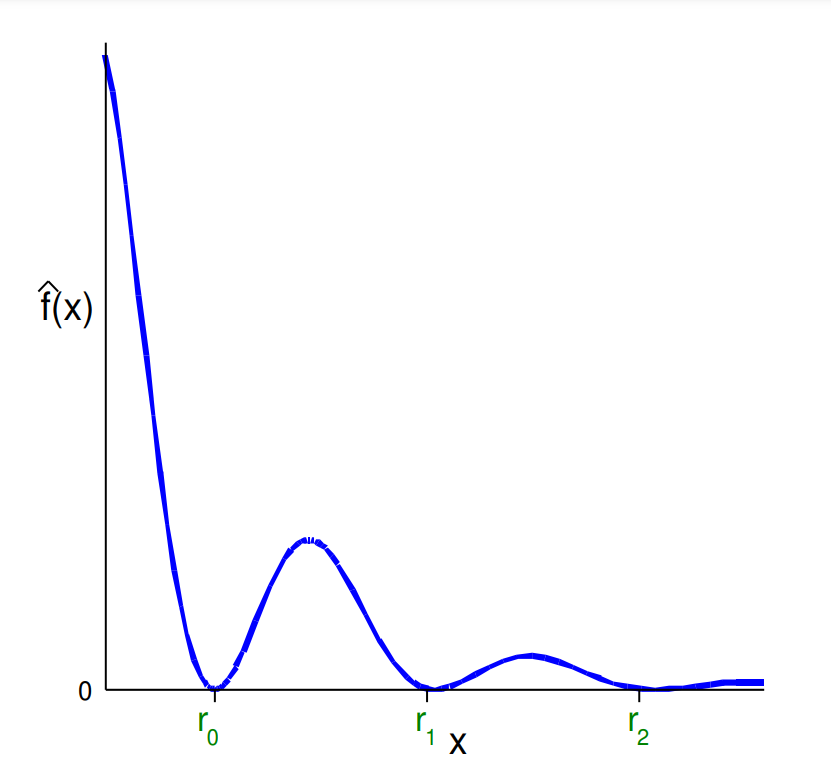
\includegraphics[width=3cm]{f2.png}
    \centering
    \caption{How $\tilde{f}$ should look like}
    \end{figure}
    
    In [Cohn-Kumar] they used a polynomial of degree $803$ and $3000$ digits of precision to find $f$ and $\tilde{f}$ which looked like this with $200$ forced double roots and $r$ very close to $2$. The key point in [Maryna] is to use a modular form with a lot of symmetries. 
    

\end{frame}



\section{Sphere packing in $\mathbb{R}^8$ by Maryna S. Viazovska}
\begin{frame}{Sphere packing in $\mathbb{R}^8$ by Maryna S. Viazovska}

The sphere packing problem in
dimension $8$

\begin{figure}[t]
    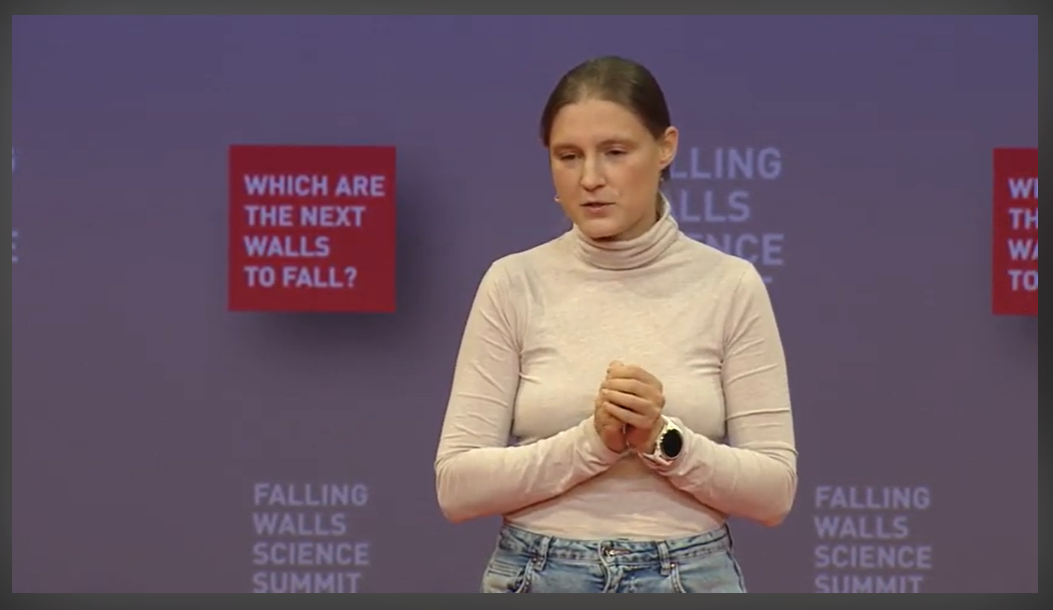
\includegraphics[width=5cm]{maryna.png}
    \centering
    \caption{Youtube video}
    \end{figure}

\href{https://www.youtube.com/watch?v=ZxT0jNzYEko}{\LARGE\beamergotobutton{VIDEO}}
\end{frame}
 

\section{Bibliography}

\begin{frame}{Bibliography}
    \bibliographystyle{unsrtnat} % We choose the "plain" reference style
\bibliography{biblio} 
\end{frame}

\section{Thanks}
\begin{frame}{Thanks for your attention :))}
\end{frame} 

\end{document}



